%!TEX root = ../scivis_lbaakman_bvanloon.tex

% \begin{figure}
% 	\centering
% 	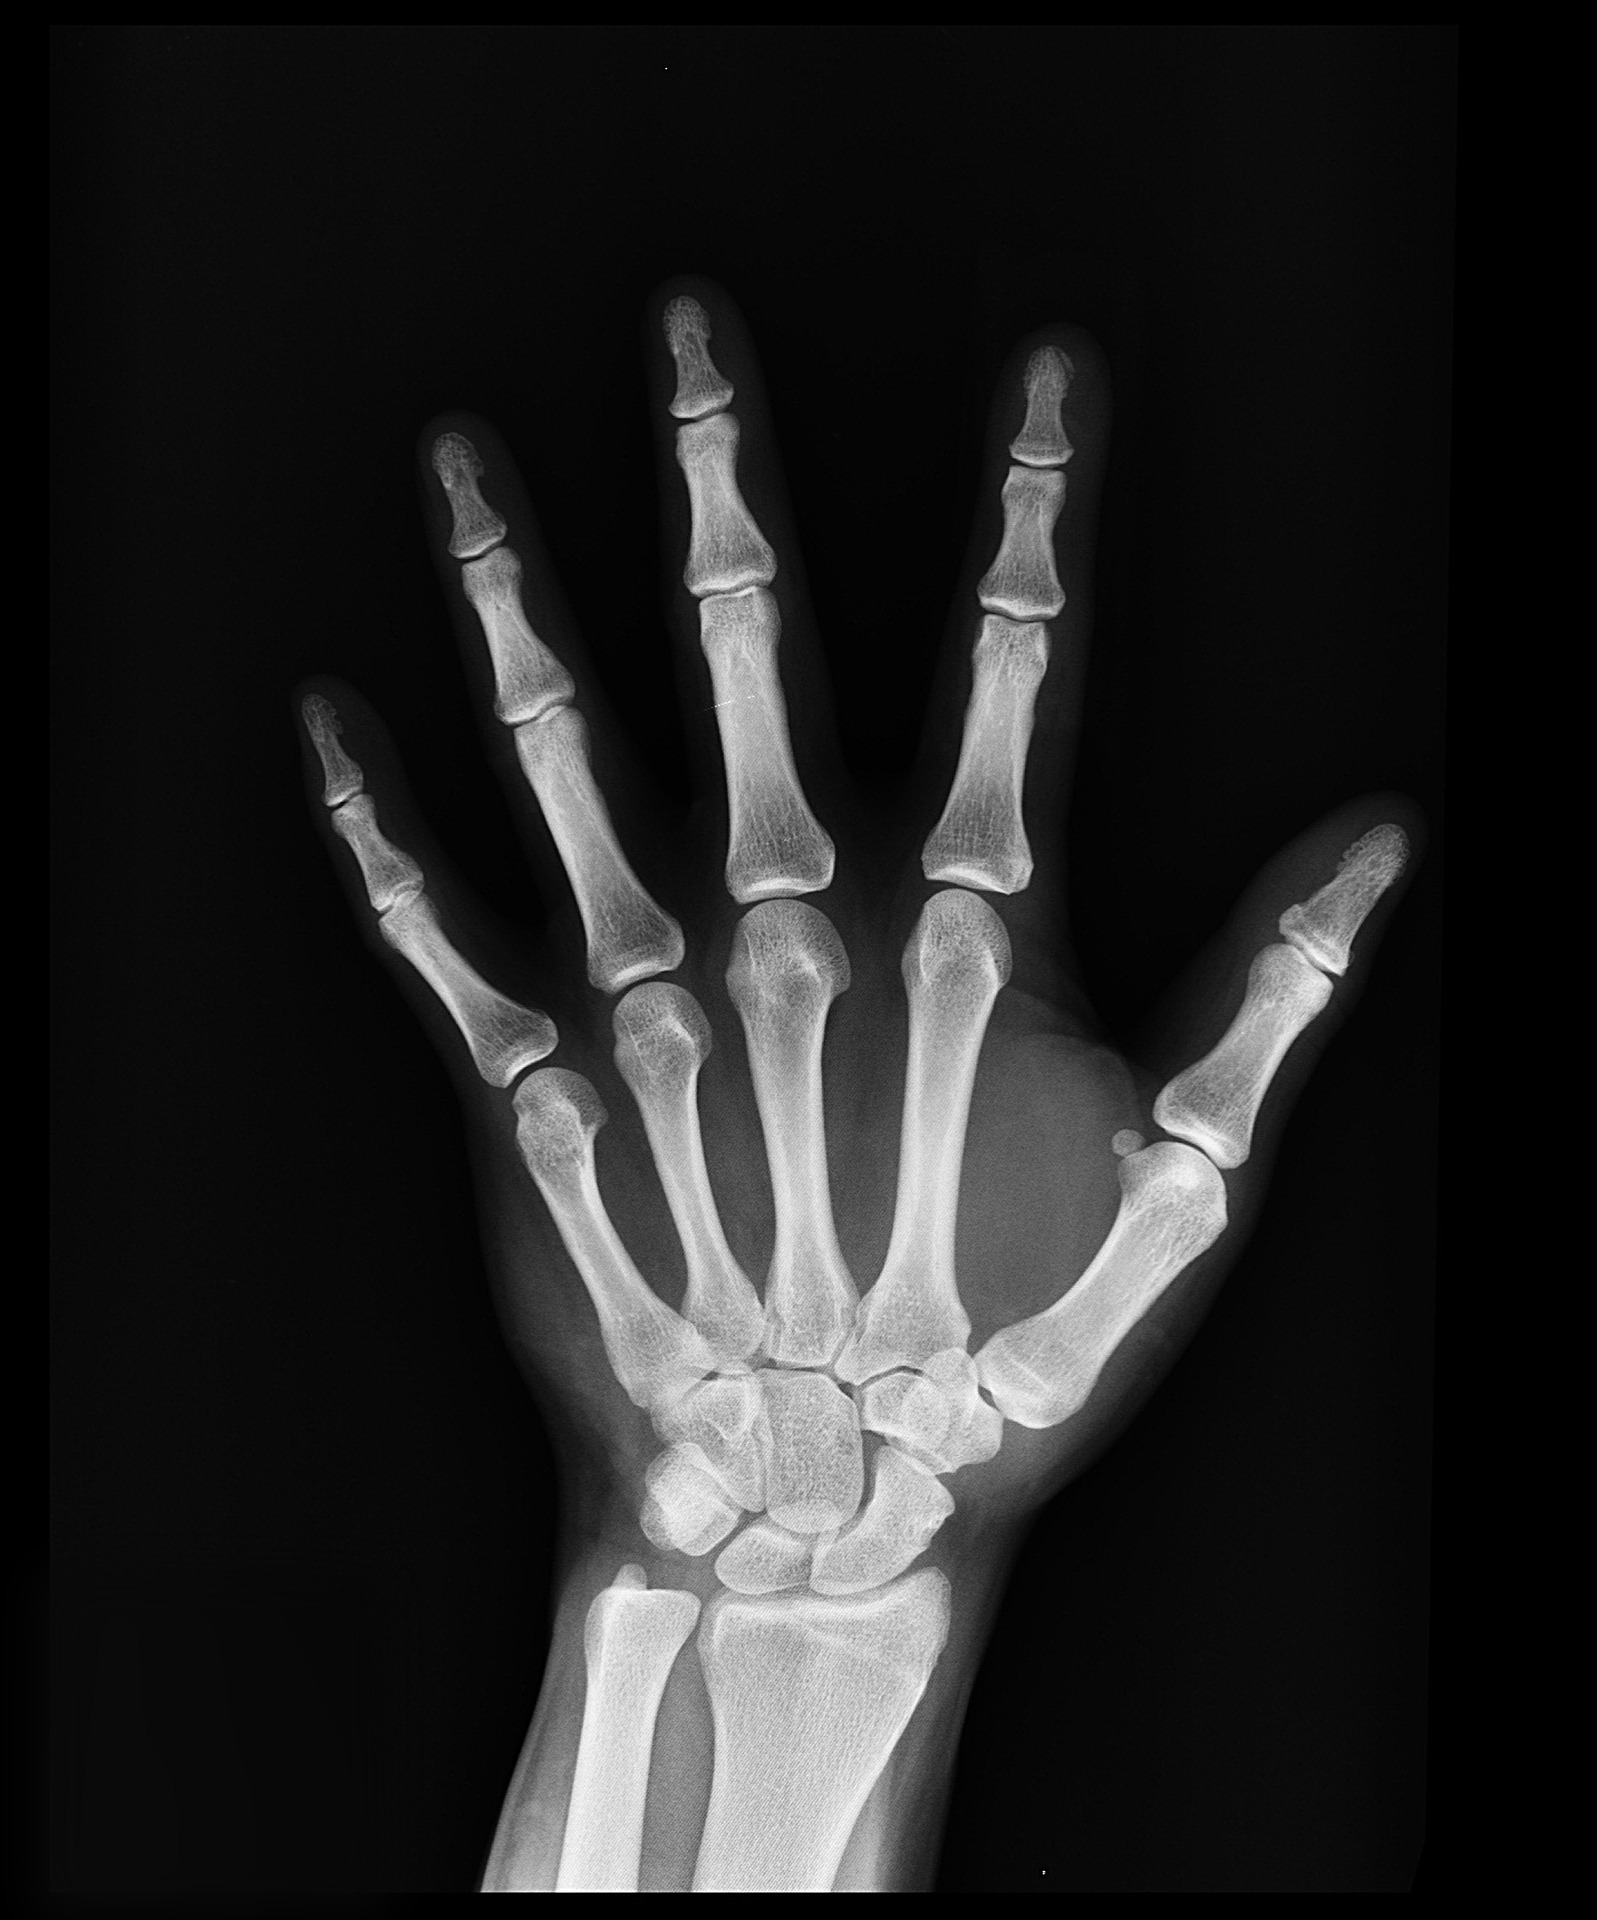
\includegraphics[width=0.5\textwidth, height=0.2\textheight, keepaspectratio]{colormapping/img/x-ray.jpg}
% 	\caption{An example of the use of a color map, image from \cite{xray}.}
% 	\label{fig:colormapping:xray}
% \end{figure}

% \Cref{fig:colormapping:xray} shows a well known example of the use of a color map. In this image lighter colors are used to indicate areas where the density of the X-rayed object are high, whereas darker colors represent areas of low density. X-rays use gray scale color maps, that is it maps the density values of the object to colors ranging from black to white. 
Colormaps are used to map scalar values to colors in order for the user to extract information about the scalar values in the visualization. The quality of a colormap can be judged by how well and intuitive the map allows inverse mapping for. Which colormap is best used in an application depends on the context and goal of the visualization. The zebra-colormap is for example well suited to visualize value variations (i.e. the first derivative of a scalar value), but would be less useful would the aim be to highlight maxima. Even historical reasons can influence the choice of colormaps. X-rays are for example displayed using a gray-scale colormap. Better alternatives might exist, but are not used due to status quo in the medical field.






\todo{Should we mention the five main goals of color maps? (Display absolute values, value ordering, value difference, selected values, and value change).}









In the next section, \Cref{s:colormaps:differentmaps}, several colormaps are discussed that are implemented in the application. For each colormap its advantages and disadvantages are given as well as a small motivation why it is included in the application. In \cref{ss:colormaps:parameterization} the parameterization of the color maps is introduced and \Cref{ss:colormaps:applying} discusses techniques that can be used to map the scalar data to the color maps. In the final section, \cref{ss:colormaps:variables}, the application of the color maps to the scalar variables in our application is discussed. 





	

